\chapter{Caminatas cuánticas sobre la línea}

\section{Primera idea}\label{IdeaOriginal}
La idea inicial de [Aarason, 1993] se basa en que hacer mediciones proyectivas a un estado en superposición es un evento aleatorio. Los pasos del caminante dependen de dicha aleatoriedad.\\

Consideremos una partícula con espín $1/2$ capaz de trasladarse en 1 dimensión (a lo largo de una línea). Su posición en $t$ se describe por un paquete de onda $\psi_{x_0}(t)$ centrado en $x_0$ y su espín $s$ se describe en la base de $\hat{S}_z$, $\{\ket{\downarrow},\ket{\uparrow}\}$. 
El espacio completo de la caminata es $\mathcal{H}=\mathcal{H}_S\otimes\mathcal{H}_P=\text{span}\left\{\ket{\sigma}\otimes \ket{\psi_{x_0}}|\sigma=\{\downarrow,\uparrow\},\,x_0\in \mathbb{Z}\right\}$. La amplitud $\ket{\Psi}$ es

\begin{equation}
    \ket{\Psi}=\alpha^{\uparrow}\ket{\uparrow}\otimes\ket{\psi^\uparrow}+\alpha^\downarrow\ket{\downarrow}\otimes\ket{\psi^\downarrow}
\end{equation}{}

en donde $\braket{\psi^\uparrow|\psi^\uparrow}=\braket{\psi^\downarrow|\psi^\downarrow}$, y $|\alpha^\uparrow|^2+|\alpha^\downarrow|^2=1$.\\

Como es usual, las traslaciones espaciales $\hat{T}$ son generadas por el momento $\hat{p}$ de la partícula, $\hat{T}=e^{-i\hat{p}l}$:

\begin{equation}
    \hat{T}_{\pm l}\ket{\psi_{x_0}}=\ket{\psi_{x_0 \pm l}}\qquad
    \begin{array}{cc}
    \hat{S}_z\ket{\uparrow}=+\frac{\hbar}{2}\ket{\uparrow}\\
    \hat{S}_z\ket{\downarrow}=-\frac{\hbar}{2}\ket{\downarrow}
    \end{array}
\end{equation}

Como hemos anticipado, la traslación de la partícula depende del espín: en la base de $S_z$, el espín arriba genera una traslación hacia la derecha y el espín abajo una traslación hacia la izquierda. Así que la evolución es generada por $\hat{U}=e^{-2i\hat{S}_z\otimes \hat{p}l}$. Sea un estado inicial $\ket{\Psi_{\text{in}}}=(\alpha^{\uparrow}\ket{\uparrow}+\alpha^{\downarrow}\ket{\downarrow})\otimes\ket{\psi_{x_0}}$,

\begin{equation}
\hat{U}\ket{\Psi_{in}}=\alpha^\uparrow \ket{\uparrow}\otimes\ket{\psi_{x_0+l}}+\alpha^\downarrow\ket{\downarrow}\otimes\ket{\psi_{x_0-l}}
\end{equation}{}

Al medir sobre el espacio de espín obtenemos el estado $\ket{\psi_{x_{0+l}}}$ con probabilidad $p^\uparrow=|\alpha^\uparrow|^2$, o el estado $\ket{\psi_{x_{0-l}}}$ con probabilidad $p^\downarrow=|\alpha^\downarrow|^2$, correspondientes a un desplazamiento $\pm l$. Después de esta medición el estado de espín queda definido arriba o abajo, por lo cual una nueva traslación tiene también un desplazamiento definido, en otras palabras, desaparece la aleatoriedad. 
Para dar el siguiente paso en forma aleatoria es necesario reponer el estado de espín superpuesto, de otra manera, el movimiento tiene la dirección única del estado de espín proyectado con la medición. Es necesario que los pasos de la caminata sean la sucesión de una traslación y la recuperación del estado de espín inicial tras cada paso. Como sea, podemos retomar el factor aleatorio del proceso si hacemos mediciones sobre distintas bases cada vez. Por ejemplo, tras haber proyectado sobre el eje $z$, una rotación de la base de medida en el ángulo $\theta$, presenta una superposición $\ket{\uparrow}=c_1\ket{\xrightarrow{}}+c_2\ket{\xleftarrow{}}$. Es equivalente una rotación del espín, a partir, por ejemplo, de la matriz de rotaciones típica $R(\theta)$\footnote{\begin{equation}
    R(\theta)=
    \begin{pmatrix}
    \cos\theta&-\sin\theta\\
    \sin\theta&\cos\theta
    \end{pmatrix}{},
    \label{MatrizRotaciones}
\end{equation}{}},

Comprobemos el resultado de $\hat{M}_zR(\theta)\hat{U}\ket{\Psi_{in}}$ donde $\hat{M_z}$ es una medición en la base de $\hat{S}_z$.
\begin{equation}
    \hat{U}=e^{-2iS_z\otimes Pl}=e^{-i(\ket{\uparrow}\bra{\uparrow}-\ket{\downarrow}\bra{\downarrow})\otimes \hat{P}l}
\end{equation}{}
Los dos términos de la exponencial conmutan, por lo cual es igual a $e^{-i\ket{\downarrow}\bra{\downarrow}\otimes \hat{P}l}e^{\ket{\uparrow}\bra{\uparrow}\otimes \hat{P}l}$. Cada exponencial se puede simplificar:

\begin{equation}
e^{\ket{\uparrow}\bra{\uparrow}\otimes\hat{P}l}=\sum_n \frac{(\ket{\uparrow}\bra{\uparrow})^n\otimes (\hat{P}l)^n}{n!}=\ket{\uparrow}\bra{\uparrow}\otimes\sum_n\frac{(\hat{P}l)^n}{n!}=\ket{\uparrow}\bra{\uparrow}\otimes e^{\hat{P}l},
\end{equation}
porque $\ket{\uparrow}\bra{\uparrow}$ es un proyector.\\

Si la longitud del paso es mucho menor que el tamaño del ancho de la función de onda, $x_0\gg l$, podemos tomar hasta primer orden en la exponencial como buena aproximación y operar:
después de que la operación está completa, es decir, la proyección sobre $\hat{S_z}$ seguido de la traslación $\hat{T}$ ya se completaron, la medición $M_z$ 

\begin{equation}
    M_zR(\theta)U\ket{\Psi_{in}}=
    \left\{
    \begin{array}{cc}
    \ket{\uparrow}\otimes(I-iPl\delta^\uparrow)\ket{\psi_{x_0}}\\
    \ket{\downarrow}\otimes(I-iPl\delta^\downarrow)\ket{\psi_{x_0}}
    \end{array}{}
    \right.
\end{equation}{}
con probabilidades, $p^\uparrow=|\alpha^\uparrow\cos{\theta}-\alpha^\downarrow\sin\theta|^2$, y $p^\downarrow=|\alpha^\uparrow\sin{\theta}+\alpha^\downarrow\cos\theta|^2$, de obtener el respectivo estado de posición.

\begin{equation}
    l\delta^\uparrow:=l\dfrac{\alpha^\uparrow \cos{\theta+\alpha^\downarrow\sin{\theta}}}{\alpha^\uparrow\cos\theta-\alpha^\downarrow\sin\theta}\qquad l\delta^\downarrow:=l\dfrac{\alpha^\uparrow \sin{\theta-\alpha^\downarrow\cos{\theta}}}{\alpha^\uparrow\sin\theta-\alpha^\downarrow\cos\theta}
\end{equation}{}

Un único paso tiene la probabilidad de ser muy grande y llevar a la partícula muy lejos, o ser mucho menor que $l$, y prácticamente no generar traslación. Como ejemplo extremo tomemos $\tan\theta=|\alpha^{\uparrow}/\alpha^{\downarrow}|(1+\epsilon)$, con $l/ \Delta x \ll |\epsilon| \ll1$. Si medimos $\ket{\uparrow}$ el desplazamiento resultante es $l\delta^{\uparrow}\approx -2l/\epsilon$.
Está claro que la caminata puede continuarse aplicando el producto $\hat{R}(\theta)\hat{U}$ $t$ número de veces, $\hat{R}^t\hat{U}^t$, sobre el estado inicial de la caminata.\\

La medición aproxima la caminata cuántica a su contraparte clásica. Vimos cómo el caso límite de medir tras cada evolución tiene resultados iguales al clásico. La medición anula las coherencias cuánticas.
Sin embargo, notemos que este nuevo proceso da como resultado una caminata aleatoria clásica, en la cual cada paso tiene probabilidad fija de ir hacia alguno de los dos lados.

\subsection{Un modelo con moneda}\label{sec:LineaInfinita}
En este modelo simplificamos las caminatas cuánticas en dos aspectos \cite{kempe2003quantum} : (1) el espacio de posiciones es discreto, y (2) las traslaciones son de magnitud constante e igual a $1$. (1) impone pensar en una partícula localizada puntualmente y no como un paquete de onda con dimensión finita, por ejemplo, comúnmente las trayectorias tienen posición inicial en $x=0$. 
Por otro lado, (2) restringe la posibilidad de traslaciones muy largas o muy cortas como encontramos en la sección anterior $\ref{IdeaOriginal}$, en cambio, las traslaciones posibles son de longitud definida e igual en todo paso. Con este modelo nos centramos en las consecuencias de las correlaciones cuánticas tras muchos pasos.\\

El espacio de la caminata se genera por dos subespacios, $\mathcal{H}=\mathcal{H}_C\otimes\mathcal{H}_P$: el de la moneda
$\mathcal{H}_C=\text{span}\{\ket{0},\ket{1}\}$, y el de la posición $\mathcal{H}_P=\text{span}\{\ket{x}|x\in \mathbb{Z}\}$. \\

Más allá de las simplificaciones, la evolución es equivalente a la de la sección anterior: lanzar la moneda y después dar un paso según el estado final de la moneda (rotar el espín y luego caminar de acuerdo al espín final). 
La evolución se da con $\hat{U}=\hat{S}(\hat{C}\otimes I)$. $\hat{C}$ opera sobre $\mathcal{H}_C$,  $\hat{S}$ opera sobre $\mathcal{H}_P$, y $\hat{U}$ opera sobre $\mathcal{H}$. Los tres son operadores unitarios.
Podemos escribir

\begin{equation}
\hat{S}=\ket{\downarrow}\bra{\downarrow}\otimes \sum_{x\in \mathbb{Z}}\ket{x-1}\bra{x}+\ket{\uparrow}\bra{\uparrow}\otimes \sum_{x\in \mathbb{Z}}\ket{x+1}\bra{x}
\end{equation}{}
$\hat{C}$ sólo opera sobre las direcciones.\\

Debido a que la definición de $\hat{S}$ es estricta y tiene una única finalidad, la cual es realizar las traslaciones impuestas por $\hat{C}$, es claro que las diversas caminatas que podamos configurar están contenidas en $\hat{C}$ y no en $\hat{S}$ (más adelante vemos que el estado inicial tiene grados de libertad equivalentes a los que introduce la moneda).
Consideremos el análisis de la caminata con el famoso operador de \textit{Hadamard}
\begin{equation}
\hat{H}=\frac{1}{\sqrt{2}}
\begin{pmatrix}
1 & 1\\
1 & -1
\end{pmatrix},
\end{equation}{}
que es una moneda equilibrada: la probabilidad de medir $\ket{\uparrow}$ ó $\ket{\downarrow}$ es $1/2$ en ambos casos. El siguiente es un paso desde el estado inicial $\ket{\downarrow}\otimes\ket{x=0}$

\begin{align}
\ket{\downarrow}\otimes\ket{0}&\xrightarrow{\;\;\hat{H}\otimes I\;\;\;}\dfrac{1}{\sqrt{2}}(\ket{\uparrow}-\ket{\downarrow})\otimes\ket{0}
\xrightarrow{\;\;\;\hat{S}\;\;\;}\dfrac{1}{\sqrt{2}}\ket{\uparrow}\otimes\ket{1}-\dfrac{1}{\sqrt{2}}\ket{\downarrow}\otimes\ket{-1}
\end{align}{}

Una medición sobre el espacio de moneda en la base $\{\ket{\downarrow},\ket{\uparrow}\}$ da como resultado la posición $\ket{x=+1}$ con probabilidad $1/2$, y $\ket{x=-1}$ con la misma probabilidad.
Para mantener las correlaciones nos abstenemos de medir a cada paso y lo hacemos sólo hasta el final. Después de 3 pasos:
\begin{align}
\ket{\downarrow}\otimes\ket{0}&\xrightarrow{\;\;\;\hat{U}\;\;\;}\dfrac{1}{\sqrt{2}}(\ket{\uparrow}\otimes\ket{1}-\ket{\downarrow}\otimes\ket{-1}\\
&\xrightarrow{\;\;\;\hat{U}\;\;\;}\dfrac{1}{2}(\ket{\uparrow}\otimes\ket{2}-(\ket{\uparrow}-\ket{\downarrow})\otimes\ket{0}+\ket{\downarrow}\otimes\ket{-2})\\
&\xrightarrow{\;\;\;\hat{U}\;\;\;}\dfrac{1}{2\sqrt{2}}(\ket{\uparrow}\otimes\ket{3}+\ket{\downarrow}\otimes\ket{1})+\ket{\uparrow}\otimes\ket{-1}-2\ket{\downarrow}\otimes\ket{-1}-\ket{\downarrow}\otimes\ket{-3}).
\end{align}{}
Si medimos ahora, ¡resulta que obtener $\ket{x=-1}$ es más probable ($5/8$) que cualquier otra posición!, inclusive la simétrica $\ket{x=+1}$. Esto es consecuencia de que sobre los valores positivos prevalece una interferencia destructiva, y en el lado izquierdo una interferencia constructiva.\\

En las posiciones y tiempos $x+t$ impares la probabilidad es siempre nula. Todas los estados en posiciones alcanzadas por la caminata, diferentes a los extremos, en el tiempo $t$ tienen amplitud igual a la suma de las amplitudes de sus primeros vecinos en el paso previo $t-1$. La amplitud de los estados con posiciones extremas provienen de un único estado previo, también extremo, y tienen amplitud $1/2^t$. 
Estas influencias se pueden comprobar directamente sobre la tabla \ref{TablaCuantica} trazando dos diagonales de pendiente $\pm1$ que corresponden a una versión simple de un cono de luz\footnote{Lo que no es sinsentido ya que la tabla corresponde a una gŕafica de espacio-tiempo $x-t$ y la velocidad de propagación de la información tiene un valor superior límite, igual a una longitud por cada paso de tiempo}: todos los valores incluidos dentro de las dos pendientes tienen influencia del valor central si sus tiempos son mayores a los de este último. De forma complementaria, la amplitud del valor central contiene las amplitudes de aquellos que para tiempos anteriores están incluidos en el cono.

\begin{table}[h]
    \centering
    \begin{tabular}{|c||c|c|c|c|c|c|c|c|c|c|c|c|}
        \hline
         &-5&-4&-3&-2&-1&0&1&2&3&4&5\\\hline\hline
        0&&&&&&1&&&&& \\ \hline
        1&&&&&$1/2$&&$1/2$&&&& \\\hline
        2&&&&$1/4$&&$1/2$&&$1/4$&&& \\ \hline
        3&&&$1/8$&&$5/8$&&$1/8$&&$1/8$&& \\ \hline
        4&&$1/16$&&$5/8$&&$1/8$&&$1/8$&&$1/16$& \\\hline
        5&$1/32$&&$17/32$&&$1/8$&&$1/8$&&$5/32$&&$1/32$ \\
    \hline
    \end{tabular}
    \medskip
    \caption{Evolución $\ket{\downarrow}\ket{0}$ con la moneda de Hadamard hasta $t=5$.}
    \label{TablaCuantica}
\end{table}

\begin{figure}[ht]
\centering
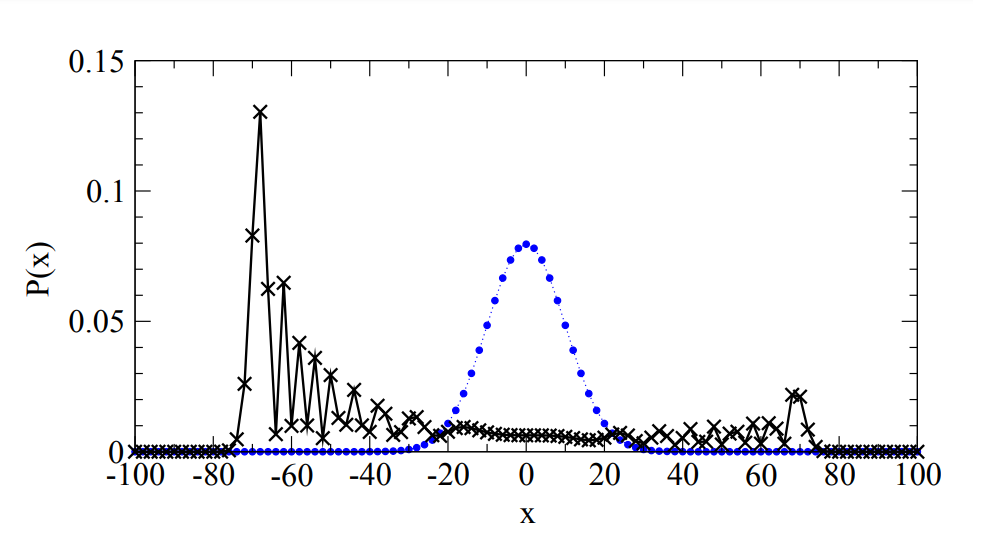
\includegraphics[width=1\textwidth]{Kap3/comparisonQW.png}
\caption{Distribución gaussiana y de la caminata cuántica tras 100 pasos. La moneda es $\hat{H}$ y $\ket{\psi(0)}=\ket{\downarrow,0}$ \cite{kendon2007decoherence}.}
\label{gr:LineaHadamard100}
\end{figure}

\subsection{Grados de libertad de la moneda}\label{sec:Moneda}
Hemos visto que la moneda balanceada de Hadamard, sin embargo, puede generar una caminata asimétrica. Hay dos formas de obtener una caminata simétrica: la primera es usando $\hat{H}$ pero partiendo de un estado inicial simétrico. La segunda es usando una moneda balanceada que incluya una fase adecuada. En esta sección comprobamos que la evolución depende de la moneda tanto como del estado inicial. Después mostramos que ambas condiciones son alternativas.\\

El estado inicial $\ket{\Psi_{\text{sim}}}=\frac{1}{\sqrt{2}}(\ket{0}+i\ket{1})\otimes \ket{0}$ hace que la caminata con la moneda de Hadamard sea simétrica. La evolución para cada estado arriba y abajo de la superposición inicial es independiente debido a la diferencia de fases. Esto se traduce en que la evolución lleva a cabo dos caminatas independientes \textit{paralelamente}, la primera con sesgo hacia la izquierda y la otra hacia derecha. Al final la probabilidad que es la suma directa de las dos caminatas tiene la forma simétrica de la gráfica \ref{gr:Hadamard100Symmetric}. \\

\begin{figure}[ht]
\centering
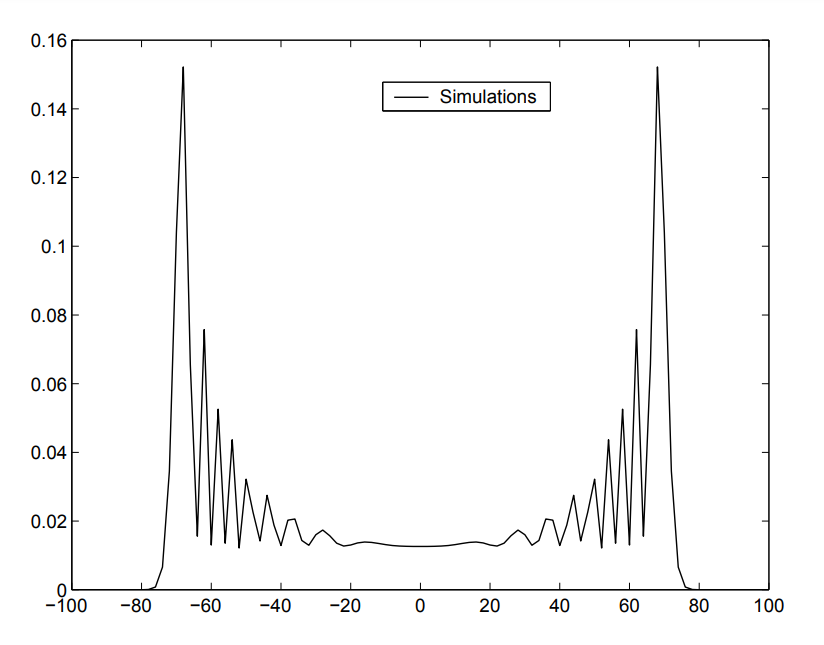
\includegraphics[width=1\textwidth]{Kap3/QWonlinesymmetricNayak.png}
\caption{Simulación de una camianata con moneda de Hadamard y estado inicial $\ket{\psi_{\text{sim}}}=\frac{1}{\sqrt{2}}(\ket{0}+i\ket{1})\ket{x=0}$, después de 100 pasos.}
\label{gr:Hadamard100Symmetric}
\end{figure}

La segunda posibilidad es usar la siguiente moneda balanceada $\hat{Y}$ sobre cualquier estado inicial en la base $\ket{\downarrow},\ket{\uparrow}$, en cuyo caso, la transformación sobre $\ket{\uparrow}$ está en desfase con $\ket{\downarrow}$ para cada paso, \cite{kempe2003quantum},
\begin{equation}
\hat{Y}=\dfrac{1}{\sqrt{2}}
\begin{pmatrix}
1 & i\\
i & 1
\end{pmatrix}
\end{equation}{}

La moneda más general en dos dimensiones tiene tres grados de libertad, restringida porque el determinante sea uno:
\begin{equation}
    \hat{C}=
    \begin{pmatrix}
    \sqrt{\rho}&\sqrt{1-\rho}e^{e\theta}\\
    \sqrt{1-\rho}e^{i\phi} & -\sqrt{\rho}e^{i(\theta+\phi)}
    \end{pmatrix}{},
    \label{MonedaGeneral}
\end{equation}{}
donde $0\leq\theta,\phi\leq\pi$ son ángulos arbitrarios, $0\leq\rho\leq1$. La transformada de fourier es

\begin{equation}
    \hat{\mathcal{F}} \hat{C}=
    \begin{pmatrix}
    \sqrt{\rho}e^{-ik}&\sqrt{1-\rho}e^{i(-k+\theta)}\\
    \sqrt{1-\rho}e^{i(k+\phi)} & -\sqrt{\rho}e^{i(k+\theta+\phi)}
    \end{pmatrix}{},
    \label{MonedaGeneral}
\end{equation}{}

\subsection{Caminos con borde}
Los caminos con borde son otro ejemplo de la diferencia entre las caminatas aleatorias clásicas y cuánticas. Recortemos la línea infinita y ubiquemos una pared absorbente que termina la caminata cuando la partícula choca con ella. Llamemos $0$ a la posición de esta pared y asumamos que el camino inicia en $1$. En el caso clásico, todos las caminatas posibles chocan con la pared, ¡ninguna la evita!. Aunque la línea es infinita y la probabilidad de recorrerla siempre hacia la derecha es diferente de cero, el análisis indica que la partícula siempre retorna y choca en $0$. Esto es equivalente a afirmar que la caminata clásica es \textit{recurrente}, esto es, que la partícula pasa por (choca) cada punto de la recta infinitas veces. La siguiente demostración se hace por recurrencia: sea $p_{10}$ la probabilidad de llegar a $0$ por \textit{cualquier} camino; en particular, sabemos que tras una iteración, la probabilidad de ir a $0$ desde $1$ es $1/2$, y un valor igual el de ir hasta $2$. Ahora nos interesa $p_{20}$ que es la probabilidad de ir a $0$ desde $2$ a lo largo de \textit{cualquier} camino. Notemos que $p_{20}=p_{21}p_{10}$.

\begin{equation}
p_{10}=\frac{1}{2}+\frac{1}{2}p_{21}p_{10} ,
\label{CaminataBorde}
\end{equation}{}
La homogeneidad del espacio hace equivalentes a todos los caminos que tienen distancia uno hacia la izquierda, en particular $p_{21}=p_{10}=p$. Teniendo en cuenta esto, la ecuación (\ref{CaminataBorde}) tiene solución para $p=1$. 
\begin{equation}
p=\frac{1}{2}+\frac{1}{2}p^2 ,
\end{equation}

En el caso cuántico el estado de posición es una superposición de las posiciones posibles. Para saber si la partícula fue absorbida en el punto $b$, se necesita hacer una medición $M_b$ en $b$ (en la pared absorbente), tras cada paso $\hat{U}$,

\begin{equation*}
    \hat{M}_b\ket{\psi}=
    \left\{
    \begin{array}{cl}
        \ket{b} & \qquad p_b=|\bra{b}\ket{\psi}|^2 \\
        \dfrac{\ket{\psi}-\braket{b|\psi}\ket{b}}{\sqrt{1-|\braket{b|\psi}|^2}} &\qquad p_{B_\perp}=1-|\braket{b|\psi}|^2 
    \end{array}
    \right.
\end{equation*}{}
Tras hacer una medición se anulan las correlaciones, que no se pueden recuperar ya que éste es un proceso irreversible. $M_b$ proyecta sobre dos subespacios, el punto $b$ solo, o su complemento. Si se encuentra la partícula en $b$ se deja de medir. [Kempe, 2003b] presenta dos protocolos útiles que llevan a la misma conclusión: ¡la partícula escapa con probabilidad $2/\pi$!